\documentclass{article}
\usepackage[utf8x]{inputenc}
\usepackage[portuguese]{babel}
\usepackage[margin=2.5cm]{geometry}
\usepackage{float}
\usepackage{graphicx}
\setlength{\parskip}{5mm}
\setlength{\parindent}{0mm}
\linespread{1.2}
\usepackage[usenames,dvipsnames,svgnames,table]{xcolor}
\usepackage{fancyhdr}
\usepackage[symbol]{footmisc}
\usepackage{amsfonts,amsmath,amssymb,amsthm}
\newtheorem{thm}{Teorema}[]
\usepackage{caption}
\usepackage[shortlabels]{enumitem}
\usepackage{verbatim}
\usepackage{listings}
\usepackage[table]{xcolor}
\usepackage{tabu}
\usepackage{array}
\usepackage{tikz}
\usepackage{url}
\def\checkmark{\tikz\fill[scale=0.4](0,.35) -- (.25,0) -- (1,.7) -- (.25,.15) -- cycle;}
\setlength{\parindent}{10mm}
\setlength{\parskip}{1mm}
\makeatletter
\newcommand{\thickhline}{%
    \noalign {\ifnum 0=`}\fi \hrule height 1pt
    \futurelet \reserved@a \@xhline
}
\newcolumntype{"}{@{\hskip\tabcolsep\vrule width 1pt\hskip\tabcolsep}}
\makeatother
\definecolor{codegreen}{rgb}{0,0.6,0}
\definecolor{codegray}{rgb}{0.5,0.5,0.5}
\definecolor{codepurple}{rgb}{0.58,0,0.82}
\definecolor{backcolour}{rgb}{0.95,0.95,0.92}
\lstdefinestyle{mystyle}{
  backgroundcolor=\color{backcolour},   commentstyle=\color{codegreen},
  keywordstyle=\color{magenta},
  numberstyle=\tiny\color{codegray},
  stringstyle=\color{codepurple},
  basicstyle=\footnotesize,
  breakatwhitespace=false,
  breaklines=true,
  captionpos=b,
  keepspaces=true,
  numbers=left,
  numbersep=5pt,
  showspaces=false,
  showstringspaces=false,
  showtabs=false,
  tabsize=2
}
\lstset{style=mystyle}
\title{\textbf{Inteligência Artificial\\Relatório 2 - Jogos com oponentes}}
\author{\textbf{Grupo 8}\\[4mm]Luís Duarte Carneiro Pinto, nº 201704025\\Sónia Das Neves Almeida, n° 201811293}
\date{\today}
\begin{document}
\maketitle
\newpage
\tableofcontents
\clearpage
\pagestyle{fancy}
\fancyhf{}
\setlength{\headheight}{30pt}
\rhead{Relatório nº2}
\lhead{\textbf{Grupo 8}}
\setlength{\footskip}{15pt}
\rfoot{\thepage}
\section{Introdução}
\hspace{10mm}Neste trabalho, vamos explorar jogos com oponentes assim como algoritmos a aplicar para o computador poder jogar contra nós. Estes tipos de jogos são caracterizados pela incerteza visto que não se sabe a jogada que o oponente fará. A diferença entre uma busca clássica e uma busca no caso de um jogo com oponente, é o tamanho do espaço de procura que é muito mais elevado no segundo do que no primeiro, porque, para saber a melhor posição para jogar, tem de explorar todas as jogadas possíveis e jogar naquela que tem mais vitórias associadas. Vamos considerar jogos com só um oponente, neste caso. Para este trabalho, utilizaremos os seguintes algoritmos:
\begin{itemize}
  \item[\textbullet]{Minimax}
  \item[\textbullet]{Alpha-beta}
  \item[\textbullet]{Monte Carlo Tree Search}
\end{itemize}
\section{Estratégias para jogos com oponentes}

\subsection{Minimax}
$\hspace{10mm}$Este algoritmo, \textit{minimax}, considera que o oponente joga sempre de maneira ótima. Desta forma, uma vez expandida a àrvore, atribui-se valores (utilidade) às folhas da àrvore que, por sua vez, vão atribuir os valores aos seus pais e estes aos seus pais e por aí adiante. A utilidade é calculada em função do jogador que queremos que ganhe. Assim, quando é a vez do computador a jogar, este vai retornar a jogada com a maior utilidade para si, enquanto que, para o seu adversário, vai calcular a jogada que minimiza a utilidade (que é a que maximiza a jogada do oponente porque o cálculo é feito em função do computador).
A árvore binária seguinte pretende ajudar a explicar como funciona o minimax:

\begin{figure}[H]
\begin{center}
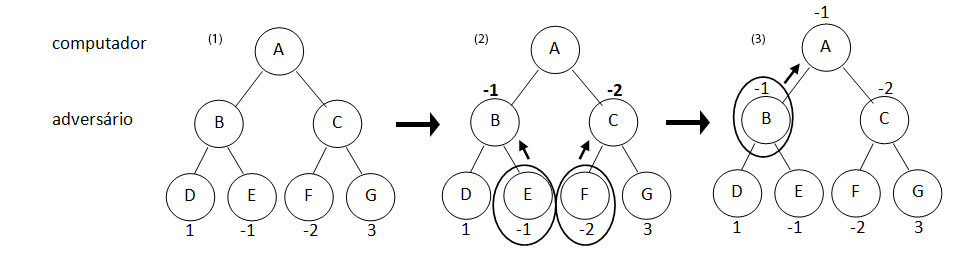
\includegraphics[scale=0.55]{figure1.png}
\caption{Esquema que demonstra o algoritmo minimax.}
\end{center}
\end{figure}

 Vamos considerar a Figura 1 para poder explicar o minimax. Comecemos por supôr que o computador joga primeiro, é análogo o caso em que o computador joga em segundo. Para saber onde jogar, deverá estimar a jogada do seu adversário. Para isso, deve simular as jogadas, calcular as utilidades da última jogada que, no exemplo, são 1 para D, -1 para E, -2 para F e 3 para G. Depois, considerando que o adversário joga de maneira ótima, deverá conservar o menor valor de utilidade de cada subárvore. Os valores conservados são -1 para a subárvore da esquerda e -2 para a subárvore da direita.


Vamos agora considerar a etapa (2) da Figura 1. O valor mínimo de cada subárvore está agora associado ao seu nó pai. Desta forma, o nó C, pai de F, tem associado o valor -2 e o nó B, pai de E, tem associado o valor -1. Agora é a vez do computador, que deve maximizar a sua jogada e escolher o valor de utilidade máximo.


Então, a utilidade associada ao nó do computador é -1, (3), e o computador irá escolher o nó cujo valor é -1 para a sua jogada, uma vez que é o melhor valor possível com aquela configuração utilizando o minimax.

Caso não haja limite de profundidade, esta estratégia é otima e completa, pois expande a árvore até não poder mais e vai considerar todos os casos possíveis.

\begin{center}
\begin{tabular}{|c|c|c|c|}
  \hline
  Complexidade & Complexidade & Completude & Otimalidade\\
  Temporal & Espacial & & \\
  \hline
  O($b^m$) & O($b\times m$) & Sim & Sim, se não for limitada  \\
  \hline
\end{tabular}
\end{center}
b - fator ramificação da árvore\\
m - profundidade ótima onde se encontra a solução

\subsection{Corte alfa-beta}
$\hspace{10mm}$Este algoritmo é idêntico ao \textit{minimax} mas com uma pequena alteração. Assim, este algoritmo deve encontrar a mesma solução que o \textit{minimax}, mas mais rapidamente porque não vai tomar em conta partes da árvore que não precisa expandir. No \textit{Alpha-beta}, o $\alpha$ está presente num nível de máximo e o $\beta$ num nível de mínimo. A grande diferença entre o \textit{minimax} e o \textit{Alpha-beta} é a expansão da árvore. No \textit{Alpha-beta}, os filhos não são gerados de uma só vez, mas um filho tem que ser gerado de cada vez para ser possível verificar se compensa continuar a explorar um dado nó ou não. O princípio de cálculo dos mínimos e dos máximos é o mesmo que para o \textit{minimax}. Vamos ver como funciona o \textit{Alpha-beta} através do exemplo seguinte. Vamos considerar que o computador é começa. A árvore só começa com o primeiro nó, A:

\begin{figure}[H]
  \begin{center}
  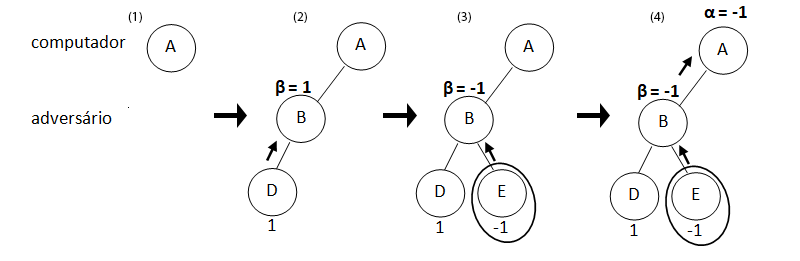
\includegraphics[scale=0.75]{figure2.png}
  \caption{Esquema que exemplifica o algoritmo alfa-beta.}
  \label{AB tree 1}
\end{center}
\end{figure}

Em (2), é executada uma busca de profundidade limitada 2, neste caso, até atingir uma folha. É, depois, calculada a utilidade dessa folha e guardado como valor provisório de $\beta$:


Agora, em (3), o outro filho de B é gerado e a sua utilidade é calculada.


O valor de $\beta$ é actualizado com a utilidade do filho E, que acabou de ser criado. O $\beta$ vale -1, em (4). O valor de $\alpha$ é, temporariamente, -1.


Agora, o segundo filho de A vai ser criado e expandido. Começa-se por criar um dos seus filhos e calcula-se a sua utilidade:

\begin{figure}[H]
\begin{center}
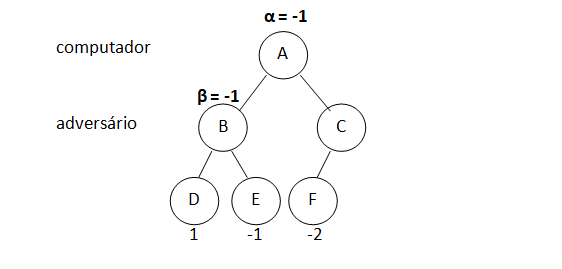
\includegraphics[scale=0.75]{figure3.png}
\caption{Estado final do algoritmo alfa-beta (seguinte à Fig.2)}
\end{center}
\end{figure}

A utilidade de F, filho de C (segundo filho de A), vale -2. Esse valor é menor que o valor de $\beta$ (onde queremos o máximo para dar esse valor ao $\alpha$), e, por isso, não vale a pena gerar o resto da subárvore com raiz C. Fica, assim, determinada a melhor jogada a realizar sem ter de expandir a árvore toda, contrariamente ao \textit{minimax}.


Tal como \textit{minimax}, é ótima e completa caso não haja limite de profundidade.
\begin{center}
\begin{tabular}{|c|c|c|c|}
  \hline
  Complexidade & Complexidade & Completude & Otimalidade\\
  Temporal & Espacial & & \\
  \hline
  O($b^m$), no pior dos casos & O($b\times m$) & Sim, se o valor de profundidade  & Sim, se não for limitada  \\
  O($b^m/2$), em geral  &                &        &                 \\
  \hline
\end{tabular}
\end{center}
b - fator ramificação da árvore\\
m - profundidade máxima explorada

\subsection{Monte Carlo Tree Search}
$\hspace{10mm}$Este algorítmo é diferente dos outros dois na medida em que tem uma componente aleatória. No início, só existe um nó. Depois, um filho é escolhido de forma aleatória. A partir desse nó, faz-se um "rollout"\footnote{Jogadas aleatórias até um estado final (vitória, derrota ou empate)}. A cada nó, fora do "rollout", é associado o número de vezes que foi explorado e o número de vitórias. Com esses dados, calcula-se um valor que nos permite fazer a seleção no próximo ciclo. Esse número é chamado Upper Confidence Bound for Trees (UCB) e vale:
\[UCB=X_j+C\sqrt{\frac{2\ln{n}}{n_j}},\text{ Onde:}\]
\begin{itemize}
  \item {$X_j=\frac{w_{j}}{n_{j}}$, $w_j$ é o número de vitórias do nó $j$ e $n_j$ é o número de vezes que esse nó foi visitado;}
  \item{C é uma constante a determinar;}
  \item{$n$ é o número de vezes que foi visitado o pai do nó $j$;}
  \item{$n_j$ é o número de vezes que foi visitado o nó $j$}
\end{itemize}

A fração entre $\ln{n}$ e $n_j$ permite que o algoritmo não seja "cego", explorando sempre o mesmo caminho mesmo que haja um caminho melhor que, por azar, foi explorado uma vez e teve uma derrota. Se um nó tem um grande número de vitórias, o algoritmo vai querer explorar mais esse nó e o UCB permite equilibrar a exploração. Em inglês, existem os termos de \textit{exploitation} e \textit{exploration}. \textit{Exploitation} tem a ver com o facto de explorar sempre o mesmo caminho por ser mais valioso. Dessa forma, a busca é mais guiada. Mas isso pode ser mau porque o algoritmo vai explorar cegamente o mesmo caminho: pode haver outro melhor que foi explorado menos vezes. A \textit{exploration} tem a ver com o facto de explorar a árvore inteira. No caso do Monte Carlo Tree Search, o UCB permite ter uma busca guiada limitada, limitando a \textit{exploitation} para mais \textit{exploration}. Este algoritmo baseia-se em quatro fases:
\begin{itemize}
  \item[\textbullet]{a seleção;}
  \item[\textbullet]{a expansão;}
  \item[\textbullet]{a simulação ( = rollout);}
  \item[\textbullet]{a propagação para trás ( = backpropagation).}
\end{itemize}

No início, a seleção é aleatória: um filho é gerado de maneira aleatória:
\begin{figure}[H]
\begin{center} 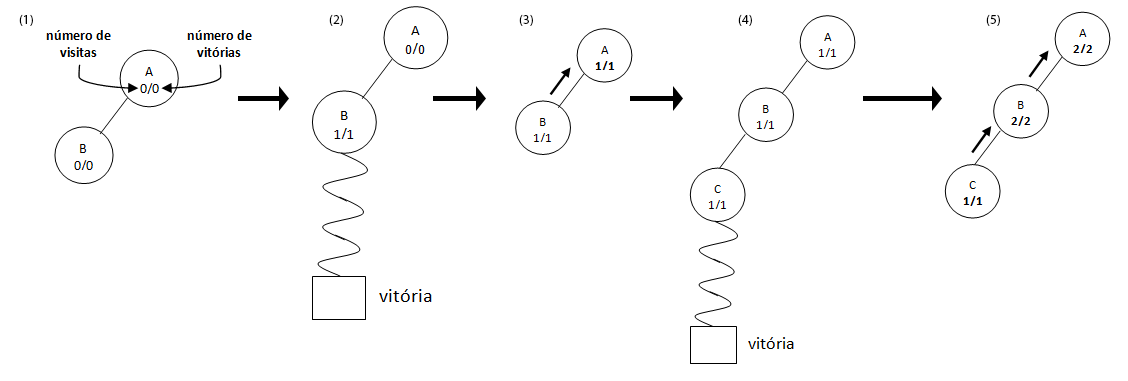
\includegraphics[scale=0.55]{figure4.png}
\caption{Esquema que demonstra o algoritmo Monte Carlo em execução.}
\end{center}
\end{figure}

No caso (1), o rollout é feito a partir do nó B. Vamos supor que o rollout determinou uma vitória. Os valores associados ao nó B são actualizados.


Na etapa (3), o valor do nó B vai permitir actualizar o valor do nó A.


A nossa árvore contém apenas dois nós, por enquanto. Para as etapas seguintes, começa-se sempre do nó raiz. Escolhe-se um nó de novo. Vamos supor que é B que é escolhido de novo para poder exemplificar a etapa de expansão. Um filho de B é gerado, aleatoriamente, C, e o rollout é feito a partir de C, fase (4).


Os valores de B e de C têm agora que ser actualizados, tal como pode ser observado em (5).


O valor de UCB permite que, depois de expandido um "irmão" de B, todos os irmãos são visitados um número semelhante de vezes, mas, mesmo assim, quanto maior o valor de UCB de um nó, maior a probabilide de ser escolhido.


\section{Sobre o connect four}
\hspace{10mm} O jogo do connect four tem como objetivo alinhar quatro "coisas" semelhantes num tabuleiro 6x7 em linha, em coluna, linha ou diagonal. \\
No nosso modelo, vamos considerar dois jogadores: X e O.
Neste jogo, a utilidade para X é calculada da seguinte maneira:

\begin{itemize}
  \item[\textbullet]{+512 se X ganhar}
  \item[\textbullet]{-512 se X perder}
  \item[\textbullet]{0 se houver um empate}
  \item[\textbullet]{-50 se houver três O e nenhum X}
  \item[\textbullet]{-10 se houver dois O e nenhum X}
  \item[\textbullet]{-1 se houver um O e nenhum X}
  \item[\textbullet]{0 se não houver token ou se houver o mesmo número de O e de X}
  \item[\textbullet]{1 se houver um X e nenhum O}
  \item[\textbullet]{10 se houver dois X e nenhum O}
  \item[\textbullet]{10 se houver três X e nenhum O}
\end{itemize}

Esses números são calculados em pares de quatro células em linha, coluna e diagonais.


\section{Algoritmos (2.1, 2.2 e 2.3) aplicados ao Connect Four}
\textbf{Implementação:} Para a implementação do algoritmo minimax, utilizamos a linguagem \textit{Python 3.7.2}.\\[3mm]
\textbf{Estrutura de Dados utilizada:} Foram utilizadas listas (em 2.1 e 2.2) para armazenar a informação (nós) de cada estado, mais especificamente cada nó associado a um valor de heurística, e dicionários no algoritmo 2.3, que será justificada a utilização, mais à frente.
\subsection{Minimax}
\textbf{Descrição: }O algoritmo \textit{Minimax} que implementamos, irá expandir um dado caminho até atingir a profundidade limite definida ou um estado final (vitória/derrota/empate). Após atingir um nó pai cujos filhos são folhas (por profundidade), irá calcular o valor heurístico\footnote[1]{A função heurística utilizada foi a descrita na secção \textit{Sobre o connect four}.} de cada um dos nós folha e, consequentemente, atribuir valor ao nó pai destas. Este processo irá ser repetido nos nós "irmãos" do referido anteriormente o que, por sua vez, irá atribuir valor ao nó pai dos pais das folhas. Este processo é repetido até se obter valor do primeiro nó filho do estado inicial e, após isto, tudo recomeça do segundo nó filho do estado inicial e por aí adiante. Utilizamos recursividade para esta implementação, uma vez que o valor de um dado nó depende do valor dos nós filhos.\\[4mm]
\textbf{Comentários: }Na implementação do algoritmo \textit{Minimax}, nós começamos por realizar uma busca em profundidade (limitada), o que não foi otimal. Após esta tentativa, falhada, procedemos ao apoio dos slides, que se encontram na bibliografia, para aumentar a eficiência. Após esta implementação, verificámos que ainda demorava algum tempo a executar para profundidades superiores a 5 e, por isso, decidimos proceder a uma última implementação que foi a implementação descrita, uma vez que foi a mais otimal. Apesar de todas estas tentativas, não conseguimos tornar o programa 100\% eficiente.
\subsection{Alpha-beta}
\textbf{Descrição: }O algoritmo \textit{Alpha-beta} é um algoritmo muito semelhante ao \textit{Minimax} mas com uma particularidade que o torna notavelmente mais rápido. Uma vez que o algoritmo \textit{Minimax} está constantemente a alterar como atribui um valor a um dado nó (máximo/mínimo/máximo/...), estando num estado de escolha de um nó de valor máximo, passando para os filhos de um destes nós (exceto o primeiro), caso o primeiro filho dê um valor inferior ao que obtivémos no primeiro nó do estado de máximo, não irá valer a pena explorar mais filhos desse nó, pois o valor dele irá ser menor ou igual ao que obtivémos em tal filho.\\[4mm]
\textbf{Comentários: }Na implementação do algoritmo \textit{Alpha-beta} tivemos de criar duas variáveis extra que não fizeram parte da implementação do algoritmo \textit{Minimax}. Estas variáveis foram chamadas de "alpha" e "beta". A variável "alpha" guardava o valor máximo temporário num nível em que se pretende maximizar a jogada e a "beta" o valor mínimo num estado em que se pretenda minimizar a jogada.
\subsection{Monte Carlo Tree Search (MCTS)}
\textbf{Descrição: }O algoritmo \textit{MCTS} é um algoritmo que utiliza pouca memória e pouco tempo de execução, caso não se exagere no número de ciclos. Utilizamos 1000 ciclos para a atribuição de vitórias/nº vezes passado no nó neste algoritmo, uma vez que o algoritmo já começava a demorar um tempo considerável para valores superiores a 1000. Decidimos utilizar dicionários como estrutura de dados visto que, na procura de valores de estados, é mais fácil procurar com um dicionário do que uma lista. Quando necessário saber quais os valores atribuidos a um dado estado, $A$, basta "chamar" por esse estado. Foi necessário o uso de uma variável temporária para guardar o caminho explorado de forma a conseguir atualizar os valores dos nós depois de realizado um dado passo.\\[4mm]
\textbf{Comentários: }Dos três algoritmos referidos, este foi aquele em que tivémos mais liberdade, uma vez que tivemos duas decisões a fazer: o valor de $C$ a utilizar (para o cálculo de UCB) e como fazer a seleção de um dado nó ao usar o valor UCB, pois os nós que não foram visitados não tem um UCB definido. Para a variável $C$ utilizamos $\sqrt{2}$, isto por razões como "a professora aconselhou" e por ter resultado bem nos testes. \\[4mm]
\textbf{Seleção dos nós: }
\begin{itemize}
\item[\textbullet]{Relativamente à selecção de nós cujo valor de UCB é 0, decidimos fazer o seguinte: Ao ser necessário realizar a selecção dum vértice filho, vai ser escolhido um número (1 ou 2) aleatoriamente. Caso o número seja 1, irá ser selecionado um nó com valor de UCB zero. Caso seja escolhido o número 2, irá ser selecionado um dos nós com o valor de UCB diferente de zero. Assim, é esperado que a cada 2 casos seja escolhido explorar um nó não visitado e um nó já visitado. Com esta forma de seleção, será provável que não se "esqueça" dum dado nó.}
\item[\textbullet]{Na seleção dum nó diante dos que tem valor UCB, decidimos escolher um número aleatório entre 0 e 1. Depois, somamos todos os valores de UCB dos diferentes nós de onde podemos escolher e vamos multiplicar esse valor pelo número gerado anteriormente. Com isto, definindo uma direção para se "ler" os nós, iremos comparar o valor que obtivemos com os diferentes valores de UCB e o nó que escolhermos será o primeiro em que a soma de todos os UCB's anteriores (com o seu inclusive) ultrapassar o valor aleatório que obtivemos.}
\end{itemize}
\section{Resultados}
$\hspace{10mm}$Na realização dos vários testes, decidimos escolher sequências de jogadas e aplicá-las a cada um dos algoritmos (com profundidades diferentes) começando pelo computador a jogar. Nas tabelas a seguir apresentadas, poderá ser observado os tempos máximos que demorou a realizar uma jogada tal como o número de jogadas e quem ganhou/se empatou. De todos os minimax que implementámos, decidimos colocar o melhor em termos de performance dos três nos dados, mesmo tendo testado todos eles.
\begin{flushleft}
  O - computador\\
  X - humano\\[4mm]
\textbf{Minimax}
\end{flushleft}
\begin{tabular}{| c | c | c | c | c |}
  \hline
  Depth & Tempo (ms) & Vencedor & NºJogadas\\
  \hline
  1 &  1    & X &  14    \\
  \hline
  2 &  13   & O &  37   \\
  \hline
  3 &  105  & X &  16    \\
  \hline
  4 &  636  & O &  27   \\
  \hline
  5 &  2063 & O &  33   \\
  \hline
\end{tabular}
\begin{flushleft}
\textbf{Alpha-Beta}
\end{flushleft}
\begin{tabular}{| c | c | c | c | c |}
  \hline
  Depth & Tempo (ms) & Vencedor & NºJogadas\\
  \hline
  1 &  2    & X &  14    \\
  \hline
  2 &  10   & O &  37   \\
  \hline
  3 &  61  & X &  16    \\
  \hline
  4 &  343  & O &  27   \\
  \hline
  5 &  1709 & O &  33   \\
  \hline
\end{tabular}
\begin{flushleft}
\textbf{Monte-Carlo}
\end{flushleft}
\begin{tabular}{| c | c | c | c | c |}
  \hline
  Depth & Tempo (ms) & Vencedor & NºJogadas & NºNós visitados\\
  \hline
  1 &  5069  & O &  7   &  1769\\
  \hline
  2 &  5128  & O &  7   &  1781\\
  \hline
  3 &  5265  & O &  7   &  1782\\
  \hline
  4 &  5335  & O &  7   &  1775\\
  \hline
  5 &  4141  & O &  7   &  1789\\
  \hline
\end{tabular}
\newpage
\begin{flushleft}
\textbf{Jogadas (Minimax e Alpha-Beta): }
\end{flushleft}
Codificando cada jogada por (A,B), onde A denota o jogador que colocou a peça e B a coluna onde jogou:\\[2mm]
Depth 1: (O,4)-(X,1)-(O,4)-(X,3)-(O,3)-(X,7)-(O,3)-(X,1)-(O,3)-(X,5)\\[2mm]
Depth 2: (O,2)-(X,4)-(O,2)-(X,2)-(O,1)-(X,7)-(O,1)-(X,3)-(O,1)-(X,1)-(O,3)-(X,4)-(O,4)-(X,3)-(O,2)-(X,3)-(O,3)-(X,4)-(O,4)-(X,4)-(O,2)-(X,1)-(O,5)-(X,1)-(O,3)-(X,2)-(O,7)-(X,7)-(O,7)-(X,7)-(O,7)-(X,5)-(O,6)-(X,6)-(O,5)-(X,5)-(O,5)\\[2mm]
Depth 3: (O,4)-(X,4)-(O,3)-(X,5)-(O,5)-(X,2)-(O,4)-(X,2)-(O,2)-(X,2)-(O,6)-(X,1)-(O,6)-(X,1)-(O,1)-(X,3)\\[2mm]
Depth 4: (O,4)-(X,4)-(O,4)-(X,3)-(O,3)-(X,3)-(O,4)-(X,1)-(O,3)-(X,4)-(O,2)-(X,2)-(O,3)-(X,2)-(O,2)-(X,5)-(O,5)-(X,6)-(O,5)-(X,1)-(O,1)-(X,1)-(O,1)-(X,5)-(O,1)-(X,2)-(O,2)\\[2mm]
Depth 5: (O,4)-(X,4)-(O,4)-(X,5)-(O,3)-(X,2)-(O,5)-(X,6)-(O,4)-(X,4)-(O,5)-(X,5)-(O,7)-(X,7)-(O,5)-(X,2)-(O,1)-(X,2)-(O,2)-(X,1)-(O,3)-(X,1)-(O,1)-(X,1)-(O,1)-(X,2)-(O,2)-(X,5)-(O,4)-(X,6)-(O,6)-(X,6)-(O,3)\\[5mm]
No \textit{Monte Carlo}, as jogadas foram diferentes mas não conseguimos tirar conclusões uma vez que foram jogadas automáticas. Como venceu todas as vezes com as jogadas pre-definidas, tentamos ganhar jogando contra ele pensando por nós próprios. Jogadas estas que podem ser econtradas dentro da pasta \textit{testes\_profundidade} nos ficheiros com nomes \textit{monte\_jogadasX.txt}.
\section{Conclusão}
\begin{flushleft}
\textbf{Minimax e Alpha Beta}
\end{flushleft}
$\hspace{10mm}$Após testar todos os algoritmos diferentes, reparamos que, tal como esperado, o \textit{Alpha beta} é uma versão melhorada do \textit{Minimax} e, portanto, jogaram ambos de igual forma mas o \textit{Alpha beta} demorou menos tempo para executar as jogadas. Como nas tabelas apenas temos a jogada que demorou mais tempo, este facto não é tão notável pelas tabelas mas foi notável na execução dos comandos (como pode ser observado nos ficheiros .txt no teste de profundidade). Reparamos, também, que depois da profundidade 4 começa a ser bastante difícil de superar o algoritmo \textit{Minimax}, o que seria de esperar porque ele vai jogar da forma mais segura para si.
\begin{flushleft}
  \textbf{Monte Carlo}
\end{flushleft}
$\hspace{10mm}$O algoritmo \textit{Monte Carlo} é diferente dos outros dois na medida em que o "estilo" de jogo que faz é mais aleatório e um estilo de jogo que fixa mais jogadas que levem o computador à vitória. Por causa deste facto, este algoritmo torna-se mais imprevisível e mais difícil de ganhar contra ele. Consequentemente, foi bastante dificil ganhar contra este algoritmo o que nos leva a crer que, contra jogadores amadores, talvez seja o mais eficiente uma vez que realiza jogadas rapidamente e ganha quase sempre. Talvez ao aumentar o número de ciclos que são feitos fosse mais difícil de ganhar contra o algoritmo  mas, devido a limitações de hardware e/ou implementação não 100\% otimal e tempo, não conseguimos testar com um número superior a 1000 ciclos.

\section{Bibliografia}
\begin{itemize}
  \item[\textbullet]{Slides aulas - \url{http://www.dcc.fc.up.pt/~ines/aulas/1819/IA/jogos_new.pdf}.}
\end{itemize}
\end{document}
